\section{Introducción}
\begin{frame}
\frametitle{Introducción}
\footnotesize
 A lo largo del crecimiento de los entornos inteligentes, como Smart House, se han realizado investigaciones con múltiples orientaciones, enfocadas en razones sociales como la comodidad y la seguridad, sin dejar de lado factores ambientales como el ahorro energético. En cuanto a una parte más técnica, estos procesos inteligentes se componen por software, hardware y firmware.\newline
 
 \begin{figure}[!]
 	\centering
 	\caption{Smart House [Imagen Propia]}
 	\label{fig:intr}
 	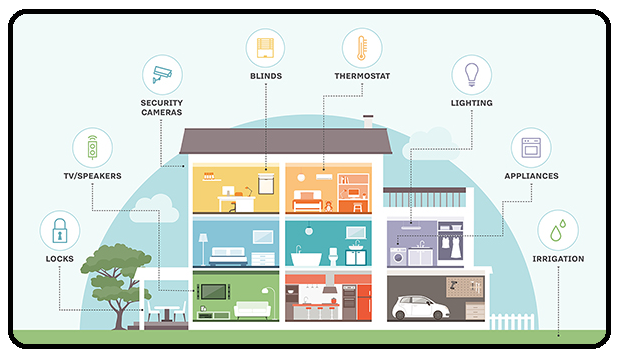
\includegraphics[width=0.4\linewidth]{Imagenes/intro}
 \end{figure}
\end{frame}